\documentclass{beamer}
\usepackage{tikz}
\usepackage{hyperref}[]
\usepackage[T1]{fontenc}
\usepackage{ctex}
\usepackage{color}
\UseRawInputEncoding

% Cannot enable in Xelatex
\usepackage{pgfpages}
\setbeameroption{hide notes} % Only slides
% \setbeameroption{show only notes} % Only notes
% \setbeameroption{show notes on second screen}

% other packages
\usepackage{latexsym,amsmath,xcolor,multicol,booktabs,calligra}
\usepackage{graphicx,listings,stackengine}

%% Enable only in Xelatex
% \usepackage{pstricks}

\author{侯悦文}
\title{Vscode Workshop}
\subtitle{代码片段,基础设置}
\institute [SSTIA] {SSTIA}
\date{\today}
\usepackage{QUT}

% defs
\def\cmd#1{\texttt{\color{red}\footnotesize $\backslash$#1}}
\def\env#1{\texttt{\color{blue}\footnotesize #1}}
\definecolor{deepblue}{rgb}{0,0,0.5}
\definecolor{deepred}{rgb}{0.6,0,0}
\definecolor{deepgreen}{rgb}{0,0.5,0}
\definecolor{halfgray}{gray}{0.55}

\lstset{
    basicstyle=\ttfamily\small,
    keywordstyle=\bfseries\color{deepblue},
    emphstyle=\ttfamily\color{deepred},    % Custom highlighting style
    stringstyle=\color{deepgreen},
    numbers=left,
    numberstyle=\small\color{halfgray},
    rulesepcolor=\color{red!20!green!20!blue!20},
    frame=shadowbox,
}

\hypersetup{
    colorlinks=true,
    linkcolor=blue,
    filecolor=blue,      
    urlcolor=blue,
    citecolor=cyan,
}
\begin{document}

\begin{frame}
    \titlepage
    \begin{figure}[htpb]
        \begin{center}
            
\includegraphics[width=0.3\linewidth]{pic/logo.jpg}
        \end{center}
    \end{figure}
    \begin{note}
        {Introduce your self}
    \end{note}

\end{frame}

\begin{frame}
    \tableofcontents[sectionstyle=show,subsectionstyle=show/shaded/hide,subsubsectionstyle=show/shaded/hide]
\end{frame}

\begin{frame}{general tips}
    \begin{enumerate}
        \item 尽可能使用英文,便于求助搜索引擎和\href{https://code.visualstudio.com/docs\#vscode}{官方文档}
        \item \href{https://jeasonstudio.gitbooks.io/vscode-cn-doc/content/}{vsocde中文文档}可能有错误且不全.
        \item 本次workshop使用windows系统作为例子,mac大多内容较为相似,部分键位不同可参考\href{https://code.visualstudio.com/shortcuts/keyboard-shortcuts-macos.pdf}{macOS快捷键}
    \end{enumerate}
\end{frame}

\section{vscode基础配置}
\subsection{vscode安装}
\begin{frame}
    安装vsocde可参考
    \begin{itemize}
        \item \href{https://zhuanlan.zhihu.com/p/264785441}{windows}
        \item \href{https://blog.csdn.net/weixin_44176432/article/details/109381781}{macOS}
    \end{itemize}
    {\color{red}记得勾选!}
    \begin{itemize}
        \item 将“通过code 打开“操作添加到windows资源管理器文件上下文菜单
        \item 将“通过code 打开”操作添加到windows资源管理器目录上下文菜单
        \item 添加到path
    \end{itemize}

\end{frame}

\begin{frame}{两种设置方法}
    \begin{itemize}
        \item UI(ctrl+,)
              \begin{itemize}
                  \item 示例:改变颜色主题
              \end{itemize}
        \item 编辑setting.json(ctrl+shift+p)
              \begin{itemize}
                  \item restore window : none
                  \item hotexit: off
                  \item "files.insertFinalNewline": true,
                  \item "files.trimFinalNewlines": true,
                  \item "editor.comments.insertSpace": true,
                  \item "editor.renderWhitespace": "boundary",
                  \item "editor.formatOnSave": true,
                  \item "editor.wordWrap": "on",
                  \item "editor.mouseWheelZoom": true,
              \end{itemize}
    \end{itemize}
\end{frame}
\subsection{JSON 文件}

\begin{frame}{JSON}
    %  \begin{itemize}%[<+-| alert@+>] % 当然,除了alert,手动在里面插 \pause 也行
    JSON(JavaScript Object Notation,JavaScript 对象表示法)是一种由道格拉斯·克罗克福特构想和设计、轻量级的数据交换语言,该语言以易于让人阅读的文字为基础,用来传输由属性值或者序列性的值组成的数据对象。尽管 JSON 是 JavaScript 的一个子集,但 JSON 是独立于语言的文本格式,并且采用了类似于 C 语言家族的一些习惯。
    JSON 数据格式与语言无关,脱胎于 JavaScript,但当前很多编程语言都支持 JSON 格式数据的生成和解析。JSON 的官方 MIME 类型是 application/json,文件扩展名是 .json。 \url{https://zh.wikipedia.org/wiki/JSON}
    % \end{itemize}
    \note {Write your notes.\\}
    \begin{note}
        {JSON是一种数据结构,它更小巧但描述能力却不差,由于它的小巧所以网络传输数据将减少更多流量从而加快速度。
        那么,JSON到底是什么?
        JSON就是一串字符串 只不过元素会使用特定的符号标注。
        JSON 是一种纯数据格式,
        ,它只包含属性,没有方法。
        JSON 的属性必须通过双引号引起来。
        JSON 要求两头有 {} 来使其合法。}
    \end{note}
\end{frame}

\begin{frame}[fragile]{JSON 示例}
    \begin{minipage}{0.6\linewidth}
        \begin{lstlisting}[language=Tex]
{
    "name": "zhangsan",
    "age": 18,
    "gender": "male"
    }
\end{lstlisting}
    \end{minipage}\hspace{1cm}
    \begin{minipage}{0.2\linewidth}
        \begin{itemize}
            \item 字符串
            \item 对象
            \item 数组
            \item 数字
        \end{itemize}
    \end{minipage}
    \medskip
    \begin{minipage}{\linewidth}
        \begin{lstlisting}[language=Tex]
{
    "students": [
        { "firstName": "san", "lastName": "zhang" },
        { "firstName": "si", "lastName": "li" },
        { "firstName": "wu", "lastName": "wang" }
    ]
    }
\end{lstlisting}
    \end{minipage}\hspace{1cm}
\end{frame}

\section{用户代码片段 User snippets}



\subsection{用户代码片段用途}

\begin{frame}{插件自带补全}
    \begin{columns}
        \column{.4\textwidth}
        \begin{figure}[htbp]
            \centering
            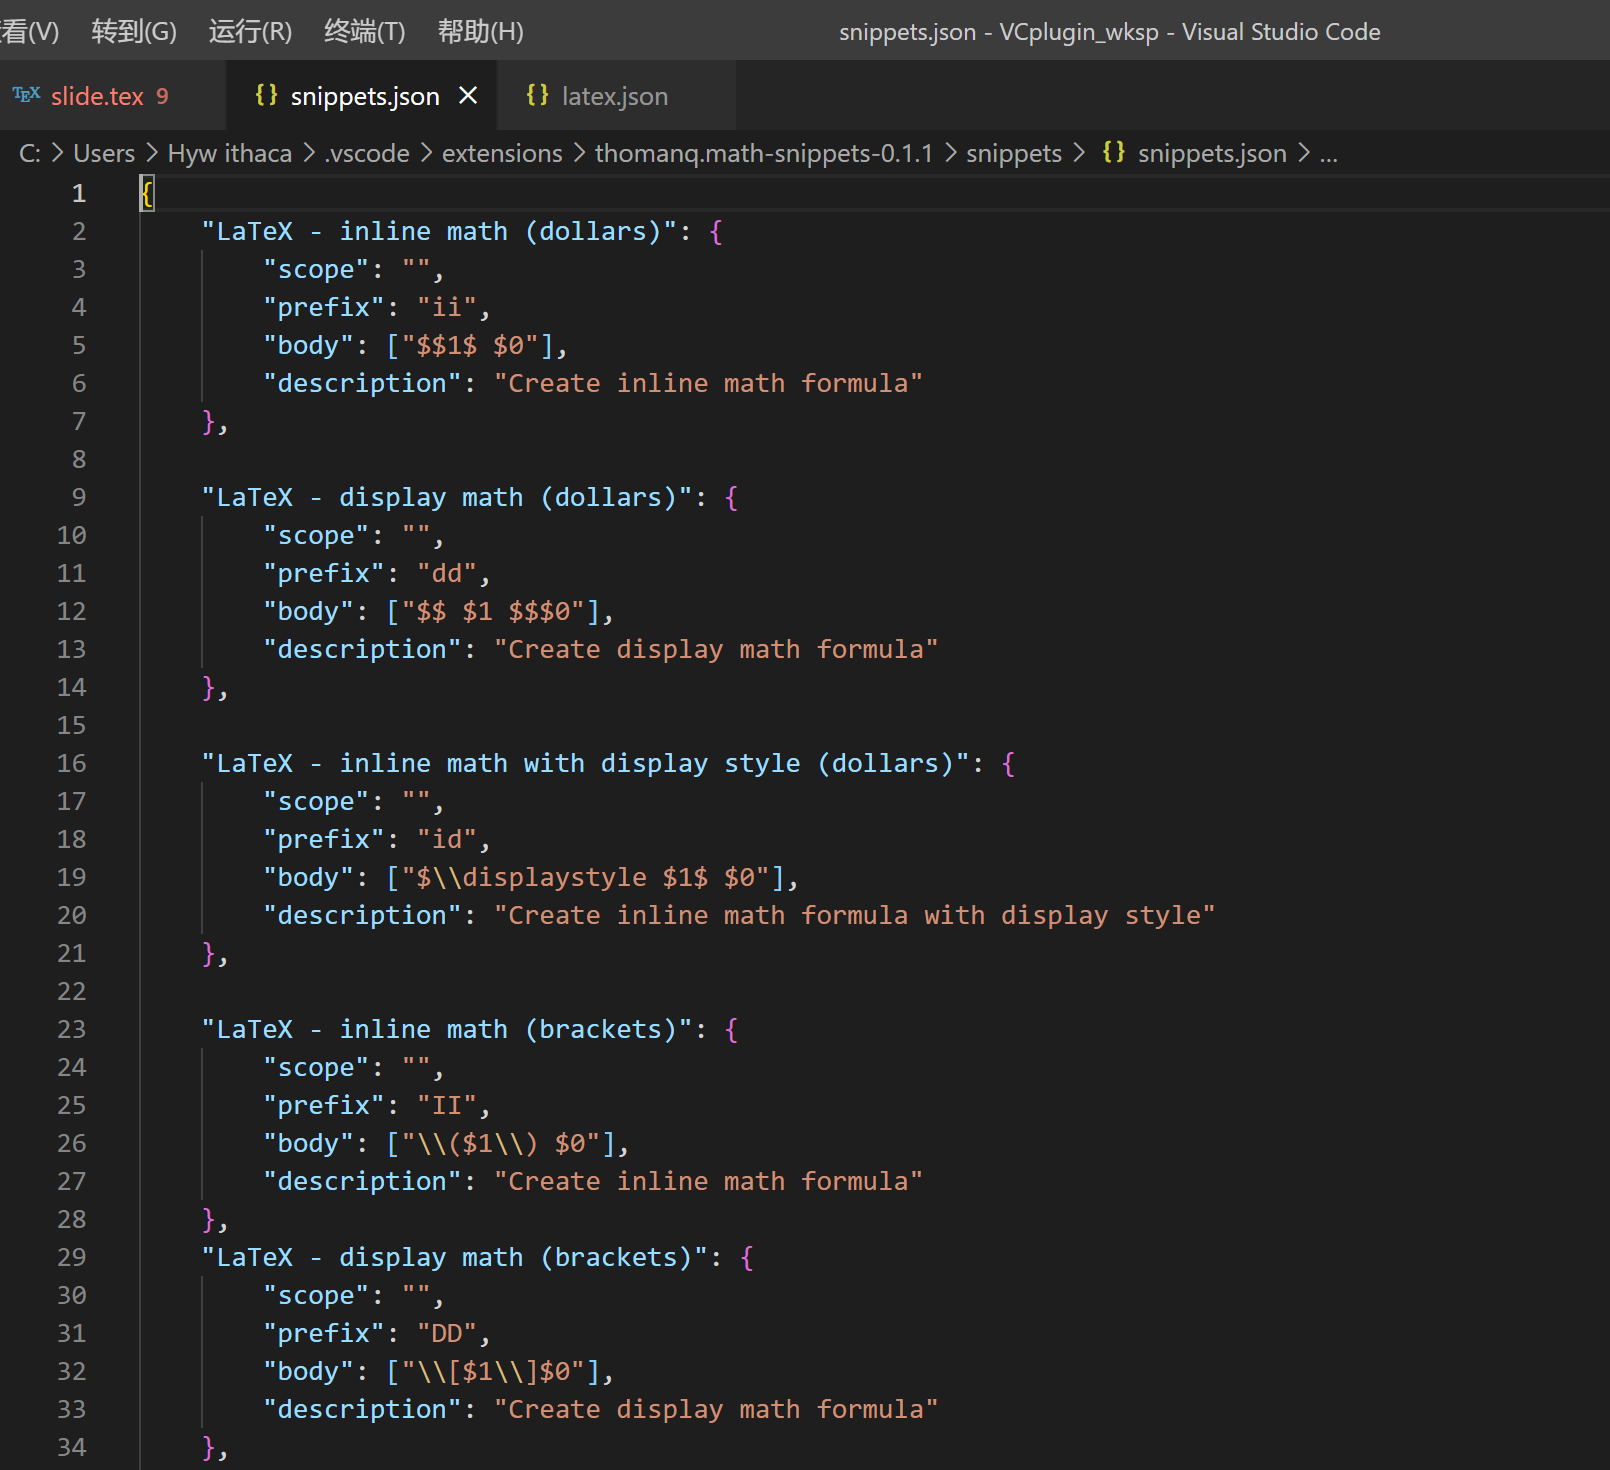
\includegraphics[scale=0.12]{pic/extension_sample.png}
        \end{figure}
        \column{.6\textwidth}
        \begin{itemize}
            \item 代码补全(定义于vscode插件)
            \item 可查看于本地$"C:\textbackslash Users<UserName>\textbackslash.vscode\textbackslash extensions\textbackslash ms-code.-\textbackslash snippets."$
        \end{itemize}
    \end{columns}
\end{frame}

\begin{frame}{添加具有代码补全功能的插件}
    \begin{columns}
        \column{.4\textwidth}
        \begin{figure}[htbp]
            \centering
            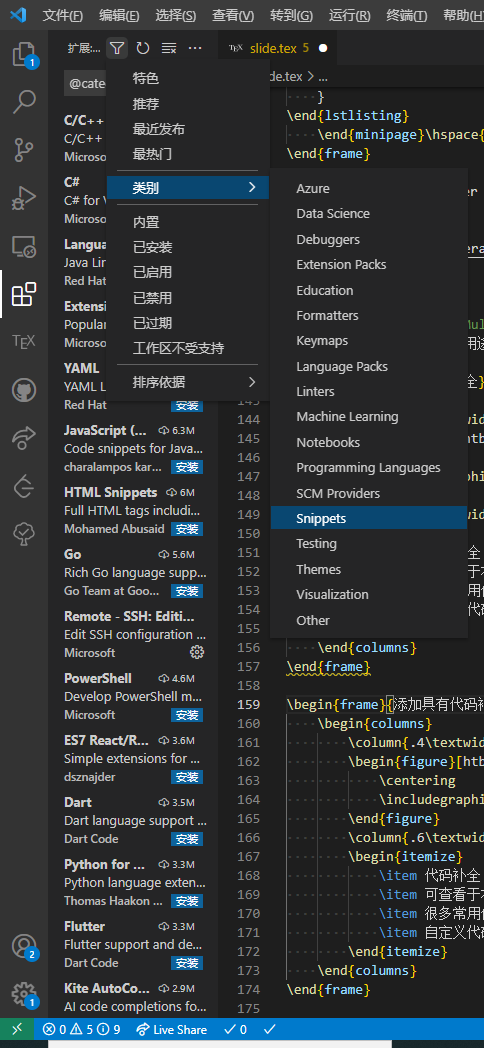
\includegraphics[scale=0.24]{pic/plugin_snip.png}
        \end{figure}
        \column{.6\textwidth}
        \begin{itemize}
            \item 在插件商店中输入关键字,并使用过滤器搜索出带有代码片段的插件安装。
            \item 很多常用代码捆绑在一起或某些补全插件中不支持
            \item 自定义代码补全
        \end{itemize}

    \end{columns}
\end{frame}

\subsection{进入用户代码片段}
\begin{frame}{进入用户代码片段}
    \begin{columns}
        \column{0.5\textwidth}
        \begin{minipage}[c][\textheight][c]{\linewidth}
            \centering
            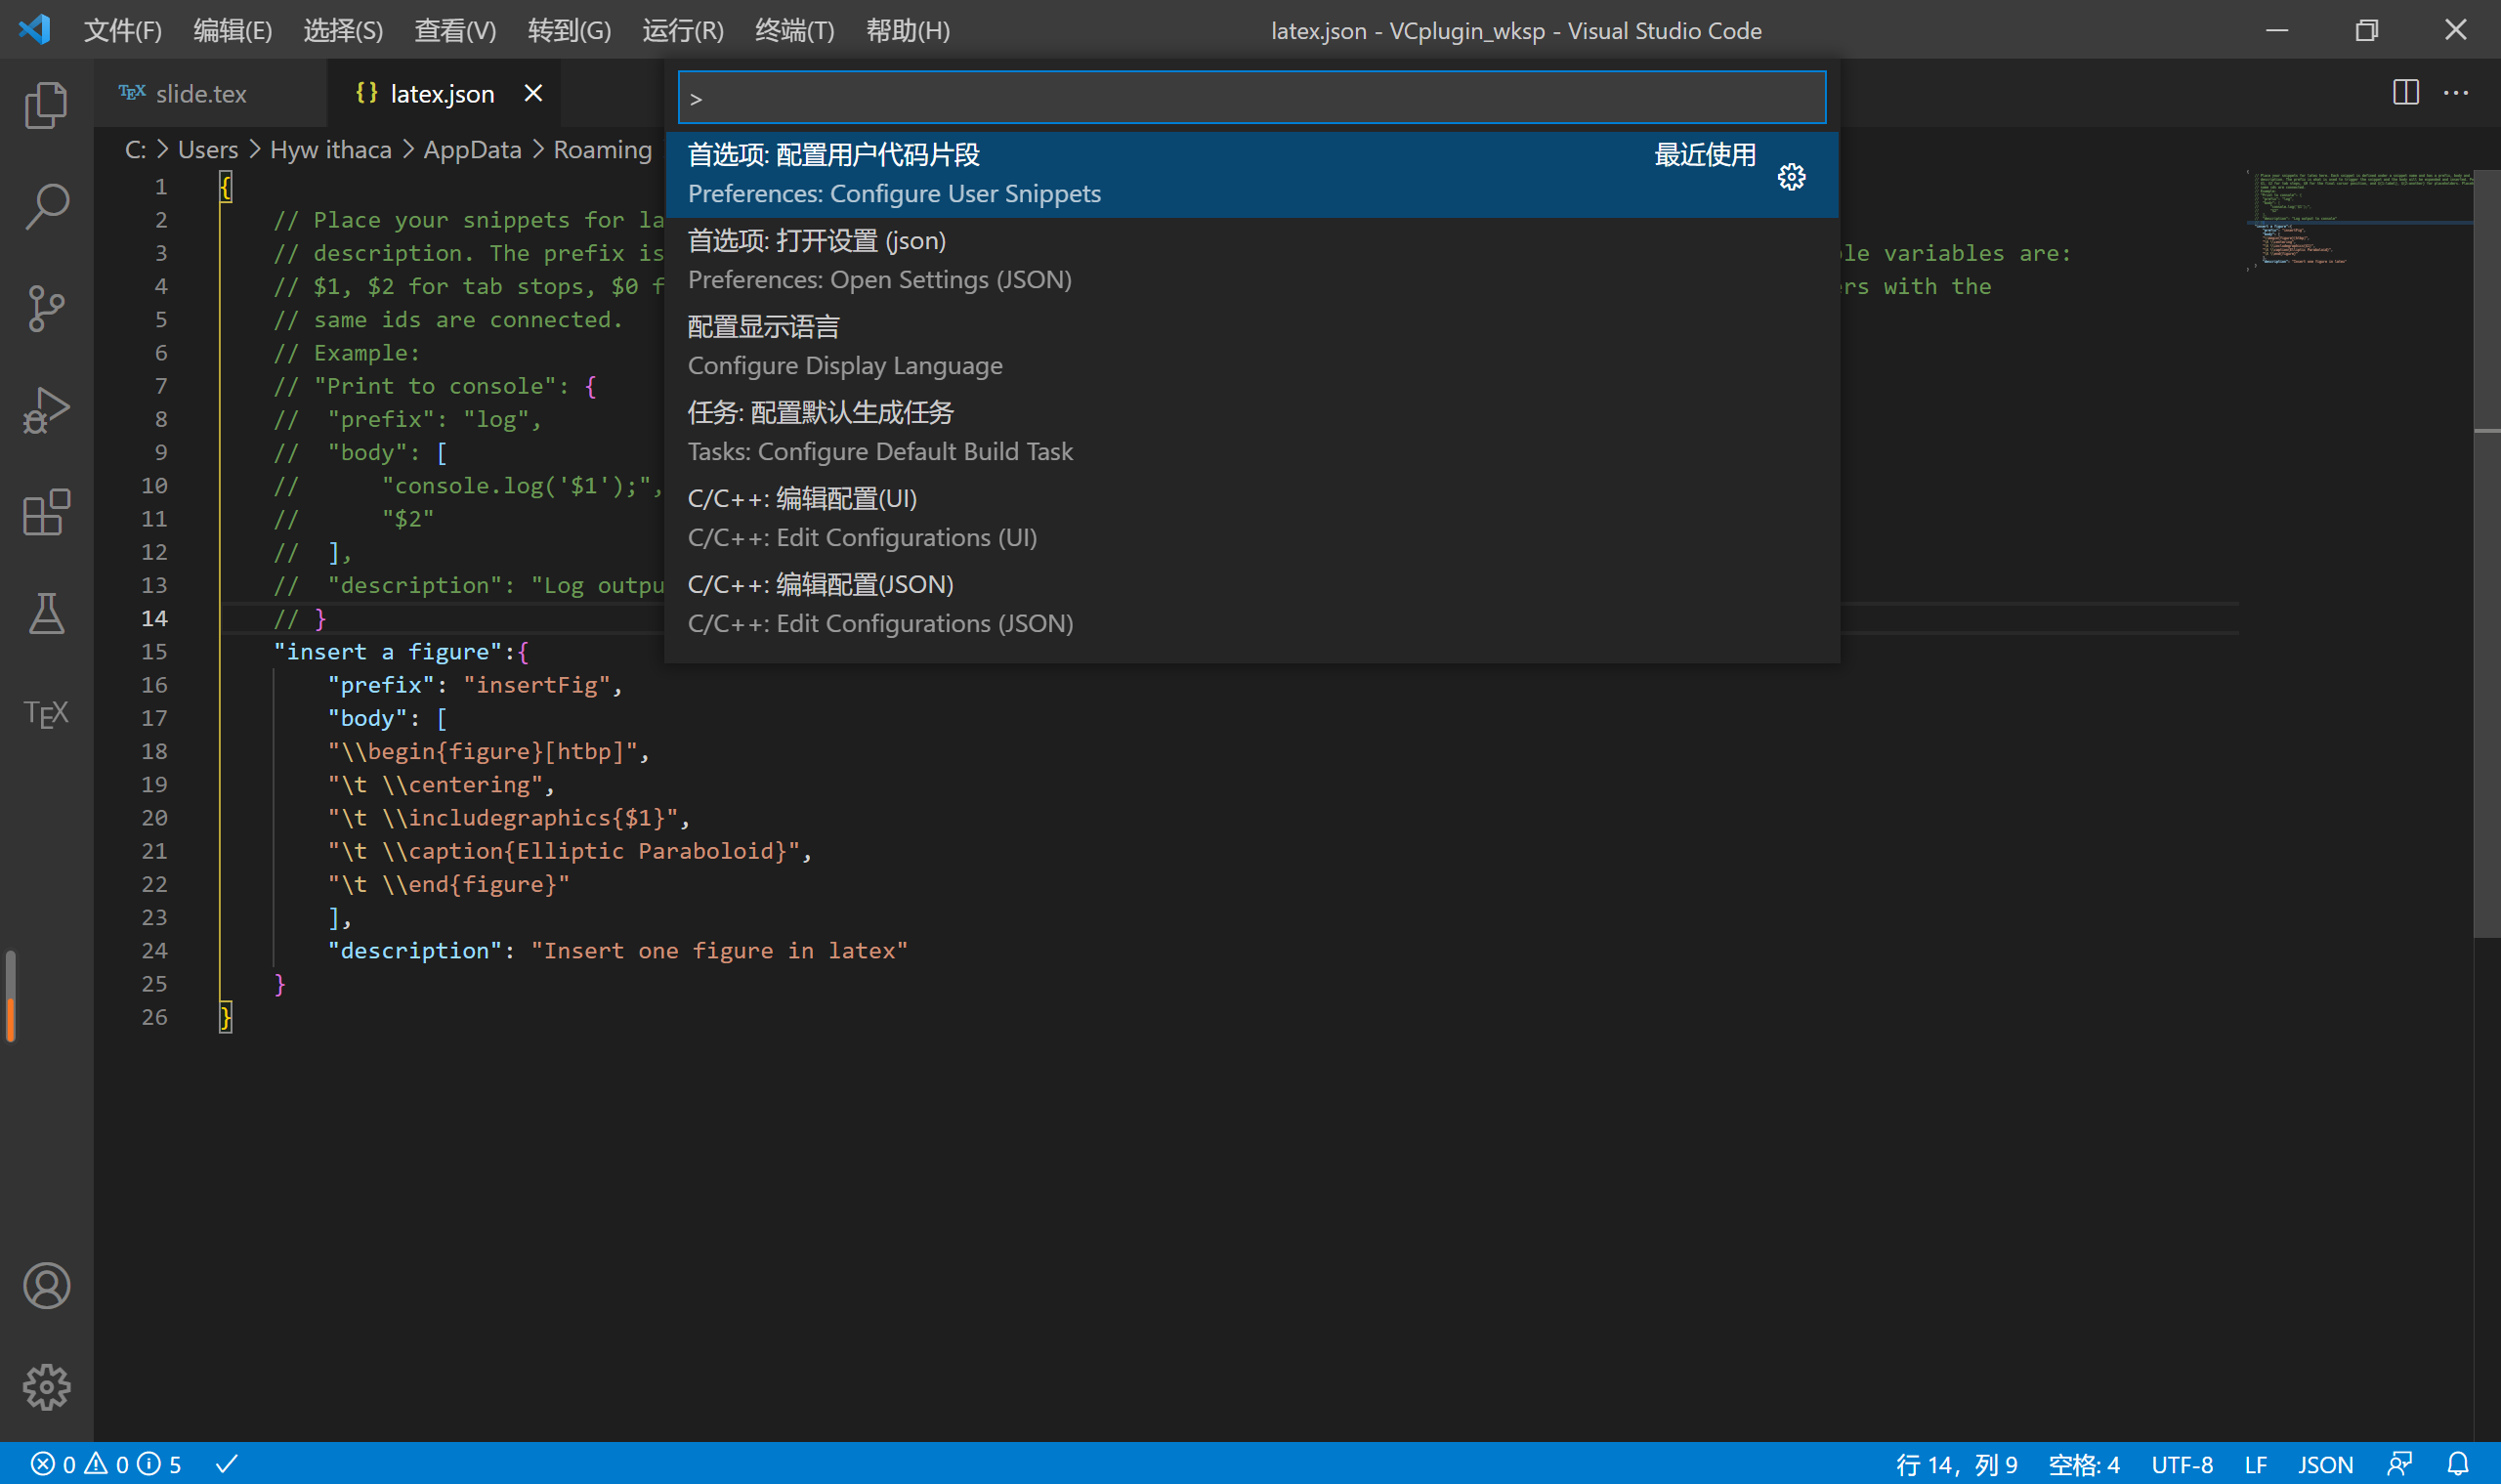
\includegraphics[scale=0.08]{pic/open.png}
        \end{minipage}
        \column{.5\textwidth}
        进入用户代码片段方式
        \begin{itemize}
            \item 快捷键Ctrl+Shift+p,然后输入snippets即可对各个文件类型进行编辑。
            \item 或图形界面操作
            \item 选择文件类型(vscode支持的语言)
        \end{itemize}
    \end{columns}
\end{frame}

\subsection{用户代码框架}
\begin{frame}{用户代码片段框架:名字与前缀}
    \begin{columns}
        \column{0.5\textwidth}
        \begin{minipage}[c][\textheight][c]{\linewidth}
            \centering
            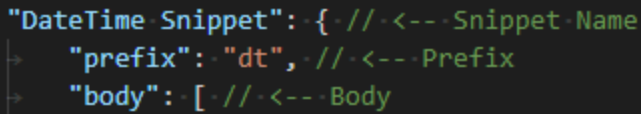
\includegraphics[scale=0.35]{pic/prefix.png}
        \end{minipage}
        \column{.5\textwidth}
        设置名字和前缀
        \begin{itemize}
            \item 前缀尽可能简明
            \item 前缀越短,使用时更方便
        \end{itemize}
    \end{columns}
\end{frame}

\begin{frame}{用户代码片段框架:主体}
    \begin{columns}
        \column{0.5\textwidth}
        \begin{minipage}[c][\textheight][c]{\linewidth}
            \centering
            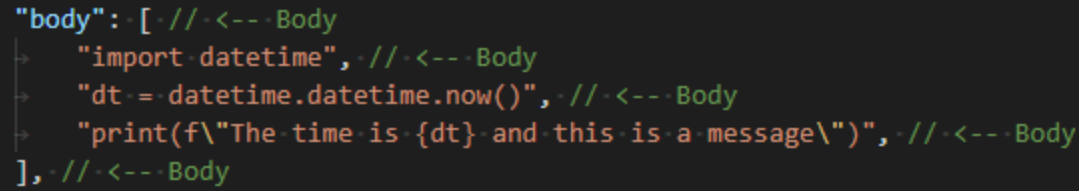
\includegraphics[scale=0.20]{pic/body.png}
        \end{minipage}
        \column{.5\textwidth}
        定义主体
        \begin{itemize}
            \item 每一行需要被双引号包裹
            \item 每一行结束需要有逗号(最后一行除外)
            \item 主体的每一行需要被中括号 \text{[ ]}包裹
        \end{itemize}
    \end{columns}
\end{frame}

\begin{frame}{用户代码片段框架:描述}
    \begin{columns}
        \column{0.5\textwidth}
        \begin{minipage}[c][.2\textheight][c]{\linewidth}
            \centering
            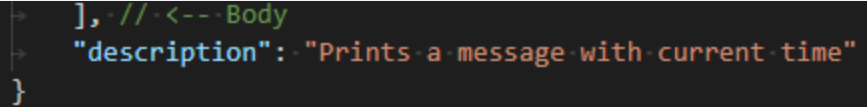
\includegraphics[scale=0.22]{pic/description.png}
        \end{minipage}
        \begin{minipage}[c][.35\textheight][c]{\linewidth}
            \centering
            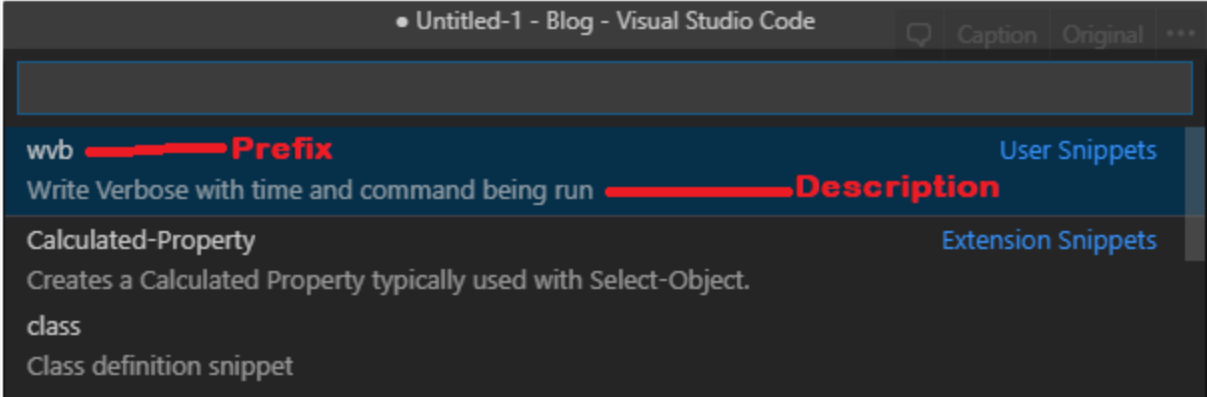
\includegraphics[scale=0.12]{pic/descritpin2.png}
        \end{minipage}
        \column{.5\textwidth}
        定义描述
        \begin{itemize}
            \item 描述片段的信息
            \item 描述会在代码片段列表中显示以便于区分
        \end{itemize}
    \end{columns}
\end{frame}

\section{用户代码片段示例}

\begin{frame}[fragile]{示例:\LaTeX}
    \begin{columns}

        \column{0.55\textwidth}
        \begin{lstlisting}[language=Tex,basicstyle=\tiny]
    "insert a figure":{
    "prefix": "insertFig",
    "body": [
    "\\begin{figure}[htbp]",
    "\t \\centering",
    "\t \\includegraphics{$1}",
    "\t \\caption{$2}",
    "\t \\end{figure}"
    ],
    "description": "Insert one figure in latex"
}
    \end{lstlisting}

        \column{.45\textwidth}
        \begin{itemize}
            \item \$ 为光标位置,按tab键移动 \$0为光标最终位置
            \item 注意要转义特殊字符
            \item  \href{https://www.tutorialspoint.com/json_simple/json_simple_escape_characters.htm}{更多转义参考链接}
        \end{itemize}

    \end{columns}
\end{frame}

\begin{frame}[fragile]{示例:\LaTeX}
    \begin{columns}
        \column{0.55\textwidth}
        \begin{lstlisting}[language=Tex,basicstyle=\tiny]
"equation of several lines":{
    "prefix":"align",
    "body": [
    "\\begin{${1|align,align*|}}",
    "\\label{$2}",
    "$0 ",
    "\t \\end{$1}"
    ],
    "description": "insert align equation"
}
    \end{lstlisting}

        \column{.45\textwidth}
        \begin{itemize}
            \item \$ 后label相同则内容相同
            \item 为光标处设置选项
            \item \$\{N|选项1,选项2[,选项]|\}
        \end{itemize}

    \end{columns}
\end{frame}


\begin{frame}[fragile]{示例:C++}
    \begin{columns}

        \column{0.55\textwidth}
        \begin{lstlisting}[language=Tex,basicstyle=\tiny]
    "myForLoop":{
        "prefix": "myfor",
        "body": [
            "for(int i = 1; i < 10; i = i++ )",
            "{",
            "${1:cout<<\"hello world\"}",
            "${2|break,continue|}",
            "$0",
            "}"
        ],
        "description": "custom for loop in cpp"
    }
    \end{lstlisting}
        \column{.45\textwidth}
        \begin{itemize}
            \item 为光标处设置默认值
            \item $\$\{1:\text{默认值}\}$
            \item 为光标处设置选项
            \item \$\{N|选项1,选项2[,选项]|\}
        \end{itemize}
    \end{columns}
\end{frame}

\begin{frame}{snippet自动生成}
    https://snippet-generator.app/
\end{frame}

\section{vscode多光标特性}
\subsection{多光标用途}

\begin{frame}[fragile]{为什么用到多光标}
    \begin{columns}

        \column{0.55\textwidth}
        \begin{lstlisting}[language=Html,basicstyle=\small]
.foo {
    Padding: 5;
    Margin: 5;
    Font-size: 5;
    }
    \end{lstlisting}

        \column{.45\textwidth}
        \begin{itemize}
            \item 将每个属性首字母小写
            \item 添加px到每行最后
            \item  {\color{red} 与多选快捷键结合使用}
        \end{itemize}

    \end{columns}
\end{frame}

\subsection{添加多光标}
\begin{frame}{使用鼠标添加多光标}
    \centering 使用鼠标:在键盘上按住 Alt,然后鼠标点在第二个“5”之前,那么第二个光标就创建好了。现在你可以看到两个光标,第二个光标比第一个要细一点。
    \begin{tikzpicture}[remember picture,overlay]
        \node<1->[xshift=0cm,yshift=-2.5cm] at (current page.center) {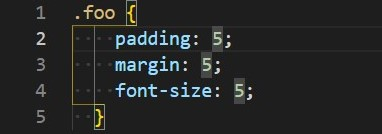
\includegraphics[height=2cm]{pic/cursor_mouse.jpg}};
    \end{tikzpicture}
\end{frame}

\begin{frame}{其他方式}
    \begin{figure}
        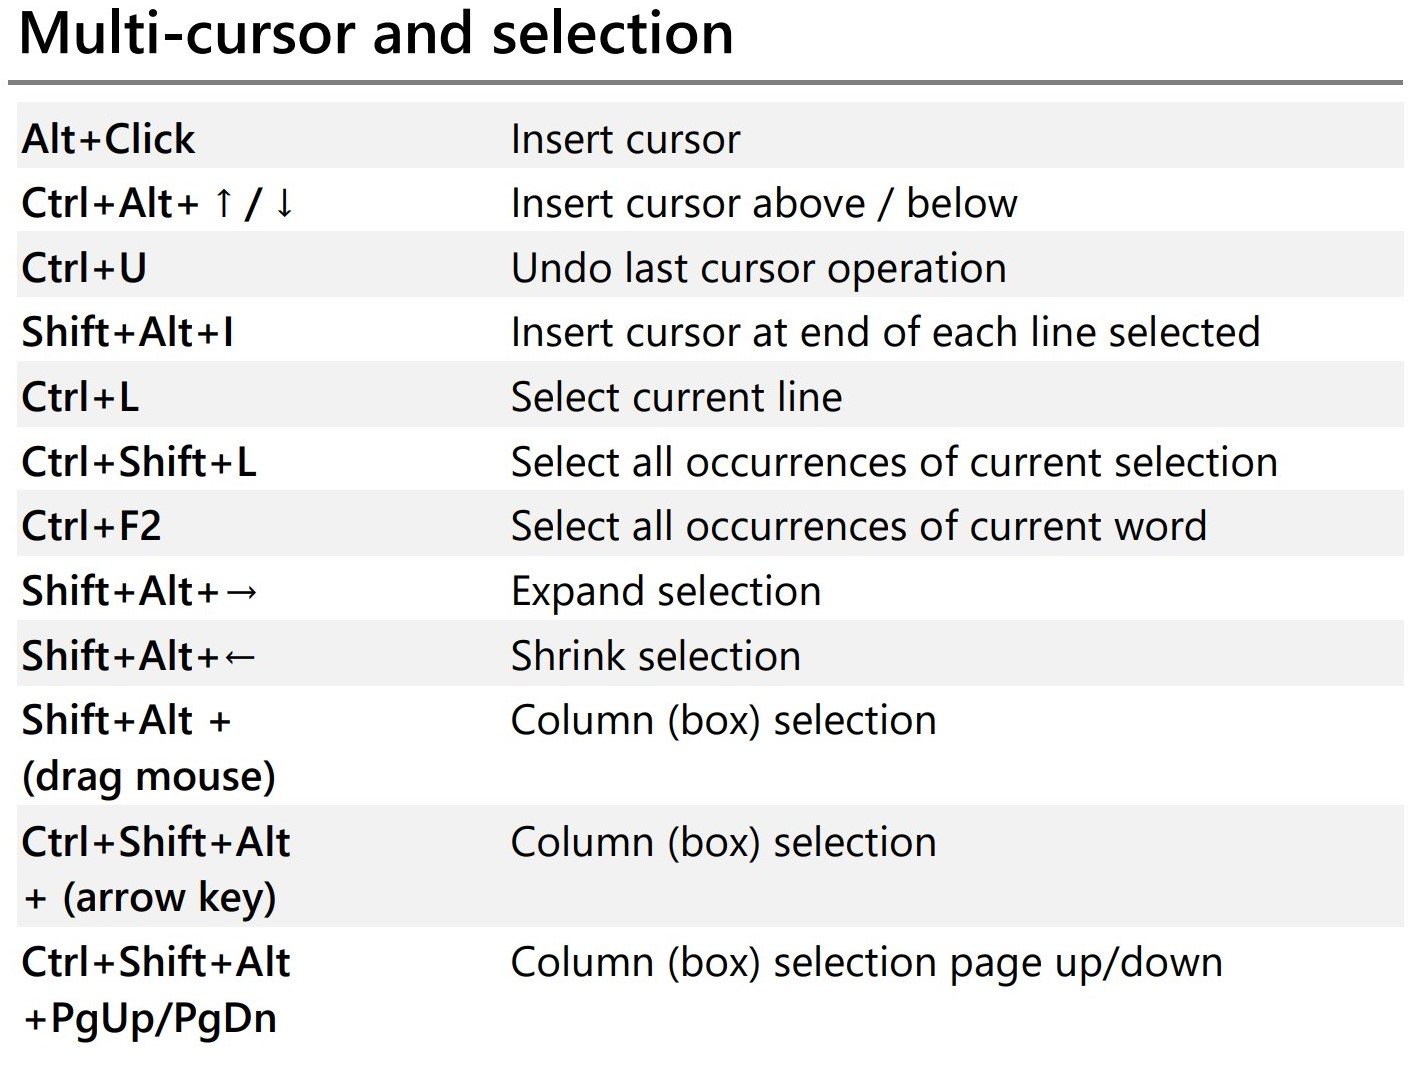
\includegraphics[scale=0.4]{pic/multi.jpg}
    \end{figure}
\end{frame}

\begin{frame}{参考}
    % \bibliography{ref}
    % \bibliographystyle{alpha}
    \small
    $https://zh.wikipedia.org/wiki/JSON$\\
    $https://www.tutorialspoint.com/json\_simple/json\_simple\_escape\_characters.htm$
    % If too many references, use this command to resize:
    % \tiny\bibliographystyle{alpha}
\end{frame}

\begin{frame}
    \begin{center}
        {\Huge\calligra Thanks}
    \end{center}
\end{frame}

\end{document}
